\newglossaryentry{exogeneity}
{name=exogeneity, 
description={An \textit{exogenous} variable $X$ does not depend on the other parameters and variables of the model. In the context of linear regression, we often refer to the assumption of \textit{weak exogeneity} the set of covariates $\boldsymbol{X}$ are considered fixed rather than variable, or alternatively that the predictor variables are assumed to be \textit{error-free}.The opposite term is endogenous}}

\newglossaryentry{lineage tracing}
{name=lineage tracing, 
description={Lineage tracing methods enable to follow the fate of individual cells in real time without interfering with their mechanistic biological functions. They are particularly useful to delineate complex biological processes involving complex, intricate cell ontology}}

\newglossaryentry{neutralisation}
{name=neutralisation, 
description={
Neutralisation is the process by which antibodies prevent viral infection of a host cell or necrosis due to toxins circulating in blood, by binding to surface proteins, thus preventing the virus from entering body cells \autocite[Figure 20a, Chapter 43]{campbell_etal20}.
On the other hand, \textit{opsonisation} fends off bacteria invasion, not by stopping the infection, but rather by promoting phagocytosis (Figure 43.20b): the two antigen-binding sites can aggregate foreign substances, easing their engulfment, while the other end-tail acts as a marker for macropahes and neutrophiles \autocite[Figure 20b, Chapter 43]{campbell_etal20}
}}

\newglossaryentry{protein-structure}
{name=Orders of protein structure, 
description={To determine the final shape, conformation and biological function of a protein, we need to apprehend 
the four potential levels of its structure \autocite{wilk-blaszczak}:
\begin{enumerate}
    \item \textbf{Primary structure:}It refers to the linear sequence of amino acids in the polypeptide chain, giving the protein's unique chemical and physical properties.
    \item \textbf{Secondary structure:} It refers to the local arrangements of the polypeptide chain, stabilised by hydrogen bonds. The most common ones are the alpha-helices and beta-sheets.  
    \item \textbf{Tertiary structure:} It is the global three-dimensional shape of the polypeptide chain, determined by the interactions between the amide backbone and the side chains attached to it: hydrogen and ionic bonds, hydrophobic interactions, and disulfide bridges.
    \item \textbf{Quaternary structure:} It details \enquote{protein complex},  formed from the combination of multiple polypeptide chains. 
\end{enumerate}
}}

\newglossaryentry{antibody}
{name=antibodoy, 
description={
Antibodies, also known as \textit{immunoglobulins} (Ig), are Y-shaped proteins composed of four polypeptide chains: two identical \textit{heavy chains} and \textit{light chains}. Each chain is additionally split into (1) a variable region at each end of the y-arm, responsible for binding to the antigen and (2) a \textit{constant region} at the stem of the antibody, which determines the  effector functions of the antibody, such as activating complement, recruiting other immune cells or neutralising toxins \Cref{fig:B-cell-receptor}.
On the other hand, the structure of the antigen receptor of T cells slightly differs, with only one antigen-binding site and only two different polypeptide chains ($\alpha$ and $\beta$). However, akin to the antibody structure, its base is a constant region that anchors the molecule in the cell’s plasma membrane, while the outer tip of the molecule is a variable region that gives the specificity of the epitope-receptor bound \Cref{fig:T-cell-receptor}. 
\begin{figure}
     \centering
     \begin{subfigure}[b]{0.45\textwidth}
         \centering
         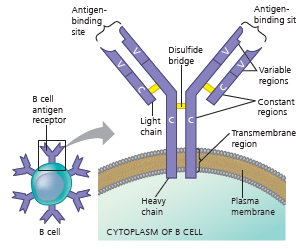
\includegraphics[width=\textwidth]{figures/B-cell-receptor.png}
         \caption{\textbf{The structure of a B cell antigen receptor}}
         \label{fig:B-cell-receptor}
     \end{subfigure}
     \hfill
     \begin{subfigure}[b]{0.45\textwidth}
         \centering
         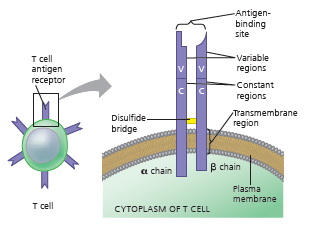
\includegraphics[width=\textwidth]{figures/T-cell-receptor.png}
         \caption{\textbf{The structure of a T cell antigen receptor}}
         \label{fig:T-cell-receptor}
     \end{subfigure}
\end{figure}
B cells can express five different \textit{classes} of immunoglobulin
(IgA, IgD, IgE, IgG, and IgM). All B cells display the same antigen receptor, known as IgD, at its surface. The four remaining have soluble forms and can be found in fluids, such as the blood, tears, saliva, and breast milk:
\begin{itemize}
    \item \textbf{IgM antibodies} They are the first deployed on the battlefield and act as an early activator of the innate immune system. They are composed of five antibodies merged together at their hips, speeding up additionally the activation of the complement system.
    \item \textbf{IgG antibodies} They are the more specialised: some are involved in \textit{passive immunity}, passing trough mother activated antibodies to the fetus, while some down regulate the activity of the innate system, preventing chronic inflammation. 
    \item \textbf{IgA antibodies} It mostly intervenes in the multiple openings of the human body, acting as a guardian of the mucous tissues: respiratory and digestive tract, sexual organs \ldots. IgA antibodies generally work by pairs, preventing access to their constant regions, and attack multiple targets by clumping them together.    
    Additionally, IgA antibodies are transmitted when mothers are breastfeeding their babies, providing them simultaneously with the breast milk. These antibodies then saturate the gut of the newborn and enforce a well-balanced microbiota.
    \item \textbf{IgE antibodies} They are involved in allergic reactions, overreacting to innocuous foreign substances, from the pollen of plants to peanuts or seafood. Originally, they used to target multicellular enemies, such as parasitic worms. But the strong development of prophylactic measures in developed countries since early 1900's deprived them from their original cumbersome enemies, and they just in turn found new irrelevant targets, a theory detailed in \autocite[Chapter 39]{dettmer21} 
\end{itemize}
The distinctive structure of an antibody is what imparts upon it its singular capacity for identifying 
with an high specificity foreign molecules, acting as a lock-and-key system. 
The antibody does not bind to the entire foreign particle, but rather to small peptide fragments commonly known as \emph{epitopes}.
B cells and circulating antibodies can directly bind to epitopes present in the extracellular medium, 
such as in the blood or lymphoid system or to antigens protruding from the surface of pathogens.
In practice, it is noteworthy that a singular antigen exposure typically triggers a diverse array of
 B cell strains, each targeting a distinct epitopes of the said antigen. This phenomenon ultimately promotes 
 an even more efficacious immune response. 
 Conversely, T cells exclusively identify antigens that are exhibited on the surface of host cells 
 via the major histocompatibility complex (MHC).}}



\newglossaryentry{transduction}
{name=cellular transduction, 
description={The set of processes and biochemical reactions by which  external signals are converted and interact with physiological activities in the cell. It involves the activation of signalling pathways, in which a signal from the environment is transmitted from one protein to another, ultimately resulting in a change in the behaviour of the cell. Cellular transduction occurs through a variety of mechanisms, including:
\begin{itemize}
    \item \textbf{Receptor-ligand interaction:} A signal molecule, called a \textit{ligand}, binds to the corresponding specific \textit{receptor} on the cell membrane, triggering a signalling cascade. The two most common signalling pathways include the G protein-coupled signalling and Tyrosine kinase signalling, in which the phosphorylation of specific tyrosine residues on intracellular proteins is induced by the bound between the ligand and its receptor.
    \item \textbf{Second messengers}: Signalling pathways often involve the activation of second messengers, such as cyclic AMP or calcium ions, which amplify the signal and coordinate a response within the cell.
\end{itemize}
The changes implied by cell signalling include regulation of the gene expression, cell growth and division, cell movement, \ldots while dysfunctional cellular transduction results in various biological disorders, including cancer and neurological diseases.}}

\newglossaryentry{cellular communication}
{name=cellular communication, 
description={Cellular communication enumerates the process by which cells coordinate their activities and functions. This communication can be either direct (e.g. through gap junctions) or indirect (e.g. through the release of signalling molecules). Generally, the intermediate signalling molecules are special proteins named \textit{hormones} (from the Greek \enquote{horman}, to excite) that circulate throughout the body. While theoretically, a given hormone could trigger any cell type, in practice it only elicits a metabolic response in the complementary target cells, that can form a complex ligand-receptor that binds the hormone specifically. This way of communication is named the \textit{endocrine system}.
The communication between cells is further classified with respect to two criteria: the type of secreting cell and the distance between the signal and its target \Cref{fig:cellular-communication}. 
\begin{figure}
    \centering
    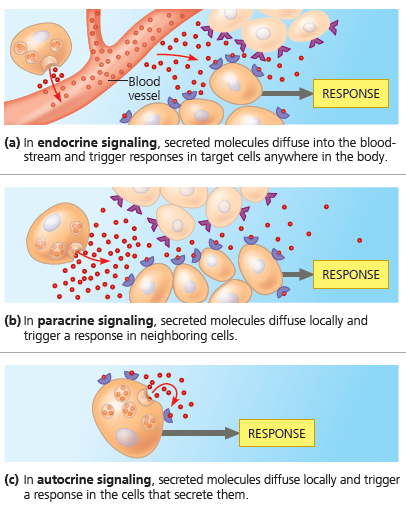
\includegraphics{figures/cell-signalling.png}
    \caption[Categories of intercellular communication.]{This figure is reproduced from ~\autocite[Fig.~45.2, p.~1000]{campbell_etal20}. Secreted molecules, in red small dots, bind specifically to a receptor protein, in purple half-arc. These receptors are either located inside cells (in that case, there is generally a direct interaction between the hormone-receptor complex and the associated biochemical process), or on the cell surface. For example, steroid-like hormones enter directly the cell, bind to an intracellular receptor protein and form a hormone-receptor complex acting as a transcription activator. On the reverse, nonsteroid hormones and growth factors only bind to cell-surface receptors and never enter the cell. Such molecules control gene expression indirectly by triggering signal \gls{transduction}}
    \label{fig:cellular-communication}
\end{figure}
}}

\newglossaryentry{metabolism}
{name=metabolism, 
description={Metabolism refers to the set of chemical reactions occurring in an organism to maintain homeostasis. These reactions are classified into two categories: catabolism and anabolism. Catabolism is the process of breaking down complex molecules into simpler compounds, releasing energy in the process. Catabolic reactions include the degradation of carbohydrates, lipids, and proteins, releasing energy conveyed by ATP molecules, that is used for cellular growth, reproduction, and movement. Anabolism is the opposite process,  building complex molecules from simpler compounds and requires energy. Anabolic reactions include the synthesis of carbohydrates, lipids, and proteins, whom some of them can be used as energy storage sources. Catabolism and anabolism work together in balance to support the needs of the organism. Imbalances in metabolism can result in various diseases, such as diabetes, obesity, and metabolic disorders.
The \textit{metabolites} are the small molecules involved in metabolic reactions within an organism, acting as bricks, end products or precursors in various metabolic pathways. The \textit{metabolome} is the complete set of metabolites present at a given time, depicting the state of cellular processes and environmental influences}}

\newglossaryentry{bioinformatic}
{name=Bioinformatics, 
description={The set of computational and statistical tools to analyse biological systems}}

\newglossaryentry{spike-in}
{name=Spike-in, 
description={Spike-in is a RNA-seq normalisation technique to account for technical variations 
that can affect the quantification of gene expression levels. Precisely, a set of artificial RNA molecules,
usually derived from foereing species and known as \enquote{spike-in controls} is added to the samples prior to the genome sequencing. 
The key steps and purposes of spike-in normalisation in RNA-seq are (\Cref{fig:spike-ins}):
\begin{enumerate}
\item \textbf{Control}: Since the spike-ins concentrations are known, they provide a reference standard
 to assess the efficiency of library preparation and sequencing across different samples or batches (indeed,
 laboratory or human variability introduced during sample preparation and sequencing can lead to differences in
 and sequencing depths between samples).
\item \textbf{Normalisation and quality evaluation}: Then, the spike-ins are used to adjust for the differences of library sizes and make
 the expression measurements across samples more comparable. 
 In addtion, the spike-ins are an indicator of the overall quality of the experiment.
 If the measured spike-in concentrations deviate significantly from their known values,
 it could suggest a strong technical issue and advocate removing the sample.
\end{enumerate}
In summary, spike-in normalization improves the accuracy  and reliability of
 differential expression analysis and other downstream analyses, by guaranteeing that observed differences
 in gene expression are biologically meaningful rather than artifacts introduced by technical biases. 
  \begin{figure}[h]{0.5\textwidth}
 centering
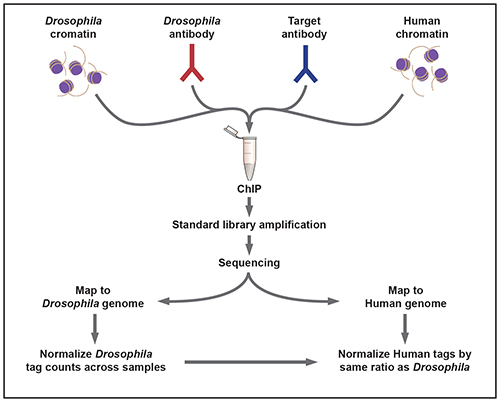
\includegraphics{figures/biological_introduction/spike-ins-normalisation.jpeg} 
\caption[\textbf{Spike-In Normalisation}]{An illustration of the RNSeq spike-in normalisation technique, by adding known concentrations
 of foreign RNA fragments to the human genome, from a reproduction of \autocite{writer16}.}
\label{fig:spike-ins}
\end{figure}
}}

\newglossaryentry{kmer}
{name=k-mers, 
description={K-mers are contiguous sequences of a given size, extracted from longer DNA sequences, 
and commonly found and shared across many indiviudals of the same species.
 Their application in bioinformatics is manifold, including \emph{sequence alignment} (
 in sequence alignment algorithms, k-mers are used to summarise and find similarities between longer DNA or RNA sequences. Using only hash tables 
 to store them, molecular biologists can identify regions of similarity at a much faster pace, comparing them only on the basis of 
 k-mer occurrence and arrangement), \emph{genome assembly} (
 in \enquote{de-novo} genome assembly, overlapping k-mers are used to reconstruct the original DNA sequence 
 by piecing them together into longer sequences to finally create a complete representation of a genome.
) and \emph{Homology Search} (To mine large sequence databases for similar sequences across numerous species, 
k-mers are efficient proxies to identify conserved protein domains) studies.
}}

\newglossaryentry{contig}
{name=Contigs, 
description={Contig are contiguous DNA sequences, assembled from overlapping DNA reads through computational algorithms,
and issued from the same origally fragmented genome. One of the main advantages of contigs is that they allow biologists to
study specific regions of the genome, even when the complete genome sequence is not available, see also glossary entry \gls{genomic-scaffolding}.
}}

\newglossaryentry{genomic-scaffolding}
{name=Genomic scaffolding, 
description={Genomic scaffolding is a crucial intermediate step in genome assembly,
designed to connect individual \glspl{contig} into larger and more complete genome sequences,
 an overview of the scales of genome reconstruction being detailled in \Cref{fig:config}.
To do so, the relative order, distance (with potential uncovered gaps) orientation of contigs must be addressed.
Genomic scaffolding is typically achieved by providing automated aligner and optimisation algorithms
 \enquote{mate-pair} (come from non-adjacent regions) or \enquote{paired-end} (sequences from opposite ends of a DNA fragment) sequences. 
 The resluting aligment is a \emph{scaffold}, namely a sequence of connected contigs with estimated gap sizes in-between. Scaffols are particularly relevant for 
biologists to get a global insight on regulatory regions and more generally on the global genomic organisation.
\begin{figure}
     \centering
     \begin{subfigure}[p]{0.4\textwidth}
         \centering
         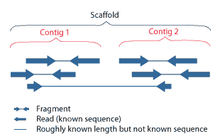
\includegraphics[width=\textwidth]{figures/biological_introduction/contig1.png}
     \end{subfigure}
     \hfill
     \begin{subfigure}[p]{0.4\textwidth}
         \centering
         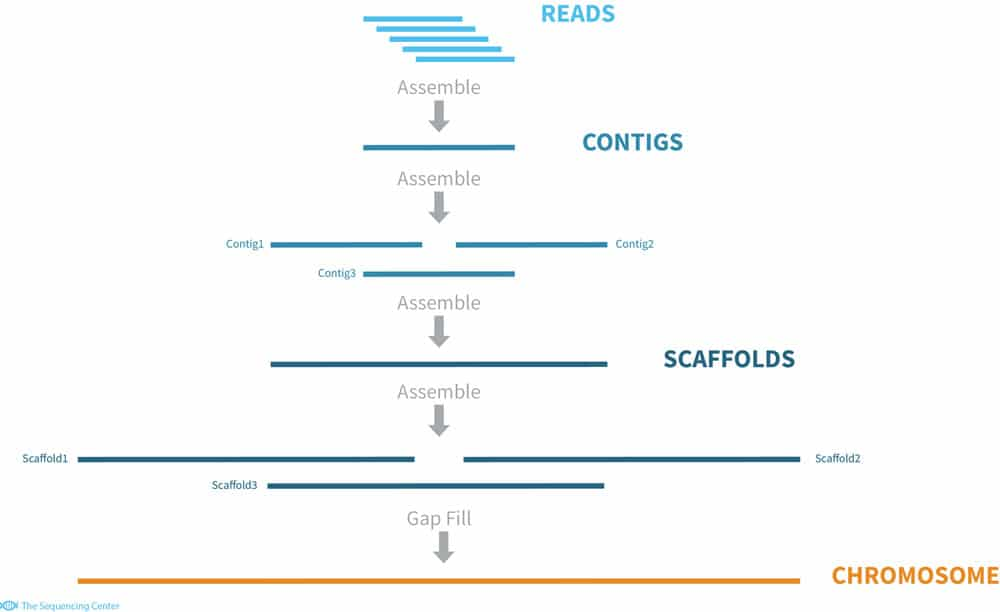
\includegraphics[width=\textwidth]{figures/biological_introduction/contig2.jpg}
         \label{subfig:contig2}
     \end{subfigure}
   \caption[\textbf{De novo Assembly Process:}]{Overlapping reads from paired-end sequencing form \textit{contigs}; overlapping contigs combined with gaps of known length form \textit{scaffolds}; sets of scaffolds are joined into a single \textit{chromosome}. Subfigures a) and b) are respectively reproduced from \autocite{california11} and \autocite[Fig.1]{What19}.}
    \label{fig:config}
\end{figure}
}}

\newglossaryentry{illumina}
{name=Illumina,
description={
While the chemical strategy underlying the core Illumina sequencing protocol has long been known, 
relying on \enquote{sequencing-by-synthesis}, a process similar to modern Sanger sequencing,
the Illumina protocol differs by its enhanced parallel sample-throughput, with the ability to 
sequence thousands of reads simultaneously thanks to its proprietary clustering and clonal amplification (see \Cref{subsec:RNASeq} 
and a comprehensive Youtube tutorial on \autocite{ambrygenetics20} for details).
 This achievement is realised through a combination of physically isolated sequencing lines coupled with the utilization
 of \emph{multiplexing}. Besides reducing the risk of introducing technical biases, early-stage multiplexing is a cost-saver by
 curtailling both reagent consumption and labor demands. Specifically, the Illumina flow cell
 incorporates eight physically segregated \emph{lanes}, enabling to process up to eight distinct samples, further extended by 
 multiplexing technique which permits the simultaneous sequencing of multiple libraries within the same lane. 
 This is accomplished by uniquely identifying each read to a sample using a specific barcode added during the library preparation, 
 the final operation consisting of assigning unequivocally each read to a sample is so-called the \emph{demultiplexing} procedure. 
 Due to the nature of the reads generated by Illumina and its prevailing market position,
 it is often referred to short-read sequencing (SRS) protocol, or Second Next Generation Sequencing, extending the historical Sanger method.
Some key features about Illumina company: they released the first sequencing tool
enable to reconstruct from scratch an entire human genome for less than $\$1000$ 
and foresees an expected $\$100$ commercial target in a near future. 
Illumina provides as well a range of highly scalable and customisable \acrshort{ngs} technologies,
ranging from the light-weight MiniSeq system targetting small laboratories
to whole-genome sequencing in populations, as part of the strategy developed in large genome centres. 
Illumina's significant status is further highlighted by its provision of a comprehensive, automated workflow
 including a range of library preparation kits.
Ultimately, Illumina provides a wide diversity of applications, covering genomic, transcriptomic or epigenomic applications,
from whole-genome sequencing(WGS) to targeted sequencing and detection of protein-binding regions (
see pdf brochure \href{https://emea.illumina.com/content/dam/illumina-marketing/documents/products/research_reviews/rna-sequencing-methods-review-web.pdf}{RNA SEQUENCING
METHODS}, \autocite[Chapter 3: Illumina DNA-to-Data NGS Solutions]{illumina23} and Wikipedia page \autocite{pasteurinstitute23} 
for a detailled review on the tools proposed by the Illumina company).
}}


\newglossaryentry{sequencer}
{name=RNASeq Sequencer platform,
description={
All three sequencing platform generation are briefly reviewed in \Cref{fig:rnaseq-generations} below:
\begin{figure}
     \centering
     \begin{subfigure}[p]{0.4\textwidth}
         \centering
         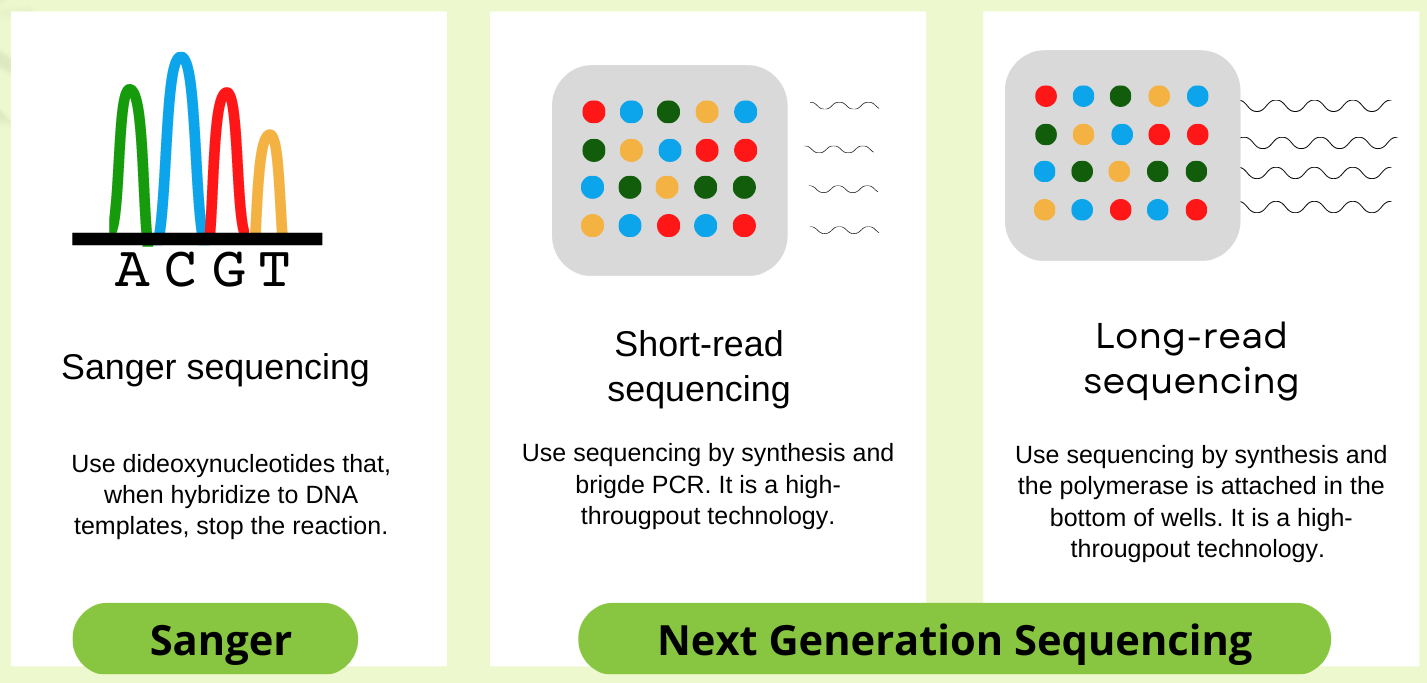
\includegraphics[width=\textwidth]{figures/biological_introduction/Different types of sequencing techniques.png}
         \label{subfig:brief-library-comparison}
         \caption[\textbf{Sequencing techniques}]{We generally classify  sequencing techniques in two categories: the historical one being the \textit{Sanger sequencing} with low throughput analysis and \textit{Next-Generation Sequencing} with much higher throughput analysis, cheaper process and often increased sequencing quality. It is further possible to set apart NGS methods into ones requiring a prior fragmentation step and focusing on sequencing short reads and ones, often referred to as the \enquote{third generation} that sequence long reads (reproduced from \autocite[Fig. 1]{gallego23}).}
     \end{subfigure}
     \hfill
     \begin{subfigure}[p]{0.55\textwidth}
         \centering
         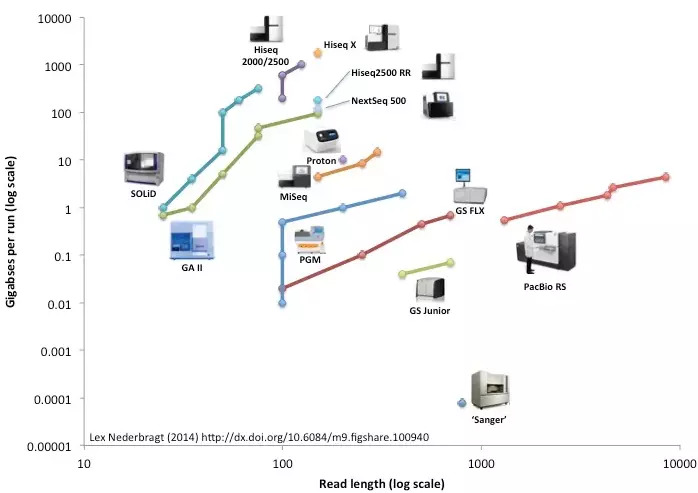
\includegraphics[width=\textwidth]{figures/biological_introduction/Difference-Between-NGS-and-Sanger-Sequencing-2.jpg}
         \label{subfig:plot-ngs}
         \caption[\textbf{Comparison of Sequencing methods}]{This scatter plot (reproduced from \autocite[Fig. 1]{dr_samanthi17})illustrates the relationship between the average length of processed sequences (representing the reading frame) on the $x$-axis and the total genome size that can be simultaneously analysed on the $y$-axis. While the traditional Sanger sequencing method allowed for long reads, its limited throughput made it impractical for sequencing the entire human genome or compiling datasets for metagenomic studies. We also note that sequencing methods must strike a balance between analysing long reads and sequencing substantial portions of the genome, although recent technological advancements are making progress in both aspects.}
     \end{subfigure}
     \vfill
     \begin{subfigure}[p]{0.95\textwidth}
         \centering
         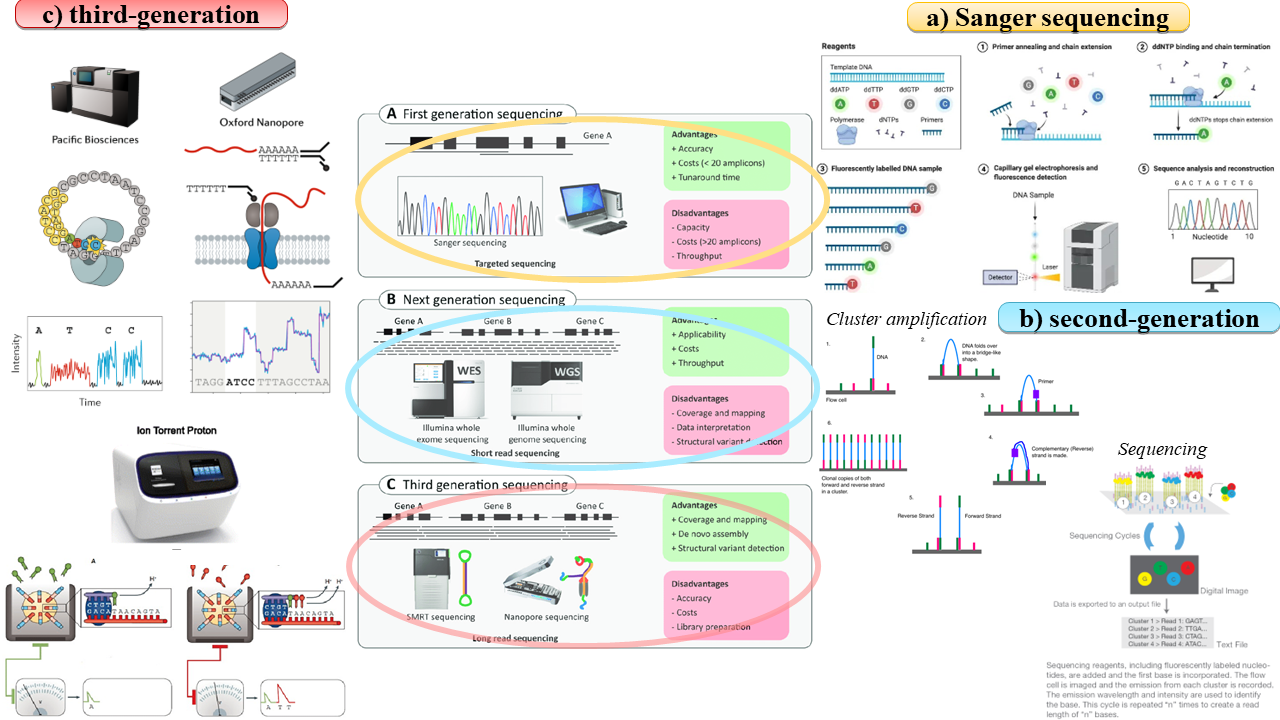
\includegraphics[width=\textwidth]{figures/biological_introduction/detailled_rnaseq_technologies.png}
         \label{subfig:detailled-techniques}
         \caption[RNASeq generations]{We illustrate key technical concepts underlying three distinct RNASeq technologies: briefly, 
		 the first generation refers to the \gls{sanger-sequencing}, the second generation to the \Gls{illumina} sequencing, reviewed in details in \Cref{subsec:RNASeq} and the \enquote{third generation} refers to a range of recent sequencing methods that share the same objective, namely sequencing long reads: \gls{pacbio}, \gls{iontorrent} and \gls{nanopore}. The central figure is reproduced from \autocite[Fig .3]{debruijn_etal21}, the Sanger workflow from \autocite[Fig .1]{shrestha22}, the \Gls{illumina} principle from \autocite{dmlapato23} and the third generation from \autocite[Fig. 1]{stark_etal19}.}
     \end{subfigure}
   \caption[\textbf{An overview of sequencing techniques, by generation.}]{}
    \label{fig:rnaseq-generations}
\end{figure} 
While both \acrshort{ngs} and Sanger techniques are nucleotide sequencing techniques, Sanger sequencing tends 
to be replaced by NGS due to its much slower sequencing ability, while being much more expensive (\Cref{subfig:plot-ngs}).
Both techniques created major outbreaks by shedding unparalleled light on complex and intertwined genetic and transcriptomics mechanisms.
It is further common to separate ngs technologies according to the average length of the reads generated,
 namely short-read (see \Gls{illumina}) and long-read sequencing (see \gls{lrs}, see Youtube tutorial \autocite{clevalab22}).
}}

\newglossaryentry{lrs}
{name=Long read sequencing,
description={ 
Long-read methods design a collection of contemporary techniques (see glossary keys \gls{pacbio}, \gls{iontorrent} and \gls{nanopore}) utilized for getting a comprehensive and preserved insight on RNA isoforms. 
It is alternatively referred to as third Generation Sequencing. Dissimilar to short-read sequencing, they do not require bridge amplification, 
instead generating long sequences from a single DNA template (hereby their alternative name of Single-molecule, real-time (SMRT) methods).
 While such methods tend to exhibit higher error rates (
up to $10\%$ inaccuracy in base calling), they are particularly well-suited for unravelling the structure of intricate DNA regions, 
such as repeats (regions comprising numerous adjacent copies of the same sequence, for instant, 
repeats account for up to $80\%$ of the genome of cereals!). The versatility and comprehensiveness of long-read based methods allows their use 
for the detection of structural variants, the building of telomere-to-telomere assemblies,
 complex genome or chromosal reconstruction, exhibiting numerous repeats or diploid organisation. For a benchmark dedicated to long-read based approaches,
 the interested reader may refer to \autocite{tlili_etal22}, paper comparing specifically the 
 Ion Torrent and Oxford Nanopore platforms. \autocite{quail_etal12} benchmarks
 specifically NGS technologies, namely the \Gls{pacbio}, \Gls{iontorrent}
 and MiSeq instrument, close to \Gls{illumina} protocol, in terms of genome coverage,
 GC bias, \acrfull{snp} and base error calling, and suggested similar performance 
 and utility for the Ion Torrent and Illumina technologies, while the lower throughput
 and higher cost of Pac Bio prohibits its use for large sequencing projects. 
}}

\newglossaryentry{pacbio}
{name=Pacific Biosciences,
description={ 
Pacific Bio comprises two main stages:
\begin{enumerate}
\item  Thousands of DNA templates are first coupled with DNA polymerase and tethered on the bottom of a nanowell.
\item The miniature camera underneath eac well captures in the second step the sequential extension of nucleotides
to the DNA templates, by measuring the resulting fluorescent reactions: when a base pairs with the DNA template,
 its signal's intensity increases.
\end{enumerate}, and is dedicated to the generation of preserved long reads 
(see \autocite{mohammed_etal22}, \autocite{nakakawa20}, \autocite{lausanne20}, 
\autocite{groot-kormelink_etal16} and \autocite{rhoads_au15} for details and concrete biological applications, 
and \autocite{haemse11} for a Youtube tutorial introduction).
}}

\newglossaryentry{iontorrent}
{name=Ion Torrent Proton,
description={ 
In this method, first, DNA templates are attached and amplified on beads, which are then loaded into wells on a semiconductor chip. 
Then, sequential addition of nucleotide to the DNA strand is detected by the induced changes in pH: precisely, when a complementary nucleotide 
is included, it releases a proton that causes a specific pH change which is detected by ion-sensitive sensors (see \autocite[Fig. 3]{kchouk_etal17}).
 This technology allows for fast sequencing of relatively short read lengths 
 (see \autocite{nguyen21}, \autocite{kchouk_etal17} and \autocite{golan_medvedev13} for details, and \autocite{bio-resource20} for a Youtube tutorial).
}}

\newglossaryentry{nanopore}
{name=Oxford Nanopore,
description={ 
After library preparation and adaptor ligation which includes a subsequent step of attaching motor proteins, 
individual DNA templates are loaded into a flowcell and dock with nanopores (tiny holes dug into the flow membrane). 
The motor protein ensures the good translocation of the RNA strand, namely that it is well-threaded through  the nanopore. 
As each nucleotide passes through, it temporarily blocks the nanopore, causing a specific and noticeable change in the electrical current. 
Precisely, the speed at which the current is blocked indicates the type of nucleotide, while its duration 
corresponds to the nucleotide's position within the DNA strand. Oxford Nanopore sequencing protocol can generate long reads of 1 to 10 kb (kilobases) size, 
however, it tends to have a higher error rate. 
By keeping the native RNA structure (no prior conversion into cDNA is required, see key \gls{library}), it has revolutionized 
personalised medecine and microbiome studies, allowing the detection of large structural variants and epigenetic modifications (
see \autocite{mackenzie_argyropoulos23}, \autocite{lin_etal21}, \autocite{maitra_etal12}
and \autocite{lu_etal16}, as well as a Youtube report on \autocite{nationaldnadatabase16}).
}}



\newglossaryentry{sanger-sequencing}
{name=Sanger sequencing,
description={ 
Sanger sequencing, also known as the \emph{chain termination method}, was first developed in 1977. Briefly, it
relies on the joint presence of modified nucleotides called dideoxynucleotides (ddNTPs) with a 
specific DNA polymerase able to resist to high temperatures. The ddNTPs lack a 3' hydroxyl group that block the 
transcription of the DNA strand. By ranking the reads generated by increasing size and identify for each of them 
the terminal nucleotide, namely identified by the ddNTP incorporated in the original DNA sequence, 
the sequence of the target DNA can be determined. 
Historically, classiyfing the reads require gel electrophoresis and manual annotation, but 
this task has since been automated through an analyser device. In addition, modern Sanger sequencing 
alleviates the integration of ddNTPs into the original genome, since the four different reactions, each 
corresponding to the addition of one of the four dideoxynucleotides, can be perfomed in one single reaction
(see also video \autocite{quickbiochemistrybasics19}, medical observatory review in \autocite{phd17},
 Wikipedia page \autocite{Sanger23} and first original mention to this technique in \autocite{sanger_etal77}).
Interestingly, while Sanger sequencing tends to lag behind other NGS technologies, 
by generating longer DNA reads and upholding a minimal error rate (
 base calling accuracy close to $99.99\%$, \autocite{shendure_ji08} ), it prevails other contemporary NGS methods,
 particularly in public health endeavors like decoding the spike protein of SARS-CoV-2 \autocite{daniels_etal21}. For 
 a more specific comparison between the closely related Illumina and Sanger sequencing methods, both using the same
 dideoxy \enquote{sequencing-by-synthesis} approach, refer to \autocite{lam_etal12}, comparing their performance for 
 the detection of insertions, deletions and single-nucleotide variants in the reconstitution of the whole human genome.
}}

\newglossaryentry{library}
{name=RNA library,
description={Briefly, the library, in the Bioinformatics fields, refers to the total collection of reads generated by a sequencing platform.
The protocol to generate this collection of sequences largely differs depending on the sequencing platform 
and the size and nature of reads generated \Cref{subfig:library-comparison-preparation}:
\begin{figure}
     \centering
     \begin{subfigure}[p]{0.4\textwidth}
         \centering
         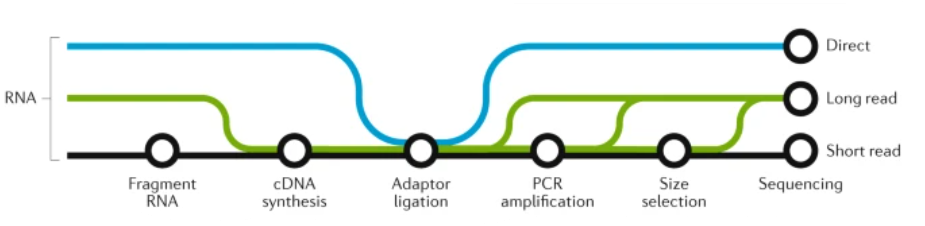
\includegraphics[width=\textwidth]{figures/biological_introduction/short_vs_long_library_preparation.png}
         \label{subfig:library-comparison-preparation}
         \caption[\textbf{Ecosystem of library preparation}]{Presented is a summary of library preparation techniques for the most common RNA-seq methods, classified with respect to the protocol preparation and the resulting sequencing opening frame into short-read (black line), long-read c(omplementary)DNA (green) or direct long-read (blue). While the intricacy and resulting technical bias differ depending on the particular approach chosen, short-read and long-read cDNA methods being the most similar in terms of library preparation, all methods involve an adaptor ligation step and are highly influenced by the quality of preservation of the biological sample (reproduced from \autocite[Fig. 1, part A]{stark_etal19}).}
     \end{subfigure}
     \hfill
     \begin{subfigure}[p]{0.55\textwidth}
         \centering
         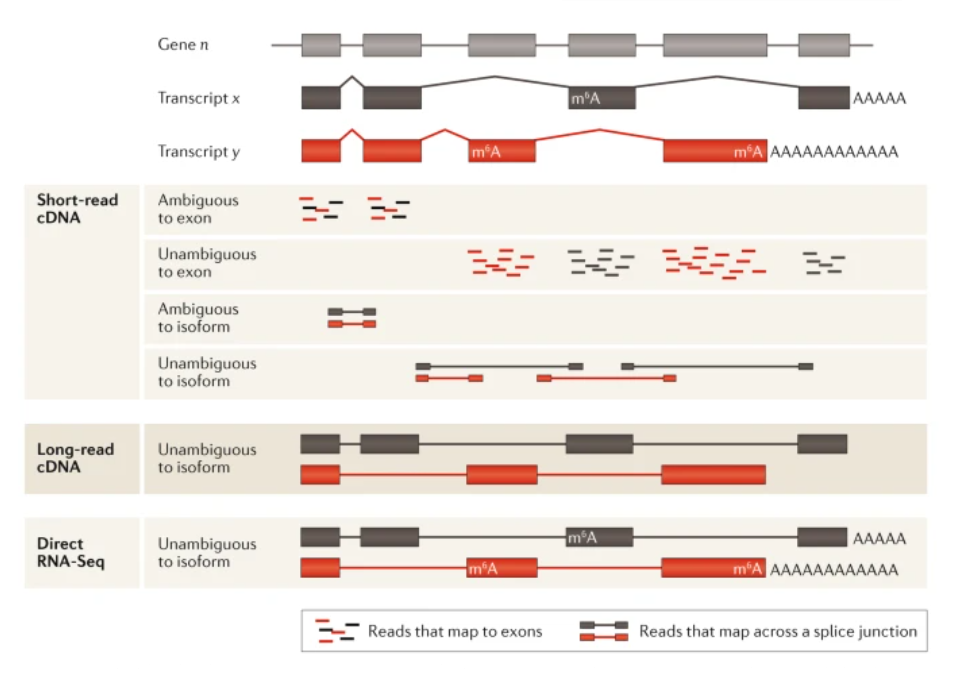
\includegraphics[width=\textwidth]{figures/biological_introduction/short_vs_long_applications_and_limitations.png}
         \label{subfig:library-comparison-limitation}
         \caption[\textbf{Comparison of short-read, long-read and direct RNA-seq analysis:}]{Over $90\%$ of human genes coding for proteins undergo alternative splicing, resulting into distinct expressed isoforms, illustrated on the top by transcripts x and y resulting from the same genetic sequence (see \Cref{subsec:alternative-splicing}).
                  More complex and detailed can be captured as we move from short-read cDNA sequencing to long-read methods that can directly sequence isoforms. Indeed, detecting isoforms with short-read cDNA sequencing is hampered by unclear mapped reads, especially when exons are shared between isoforms; in addition, reads spanning exon-exon junctions only improve isoform analysis if the junctions are not shared across isoforms. 
          Long-read cDNA methods, by returning the complete isoform in a single stage, largely alleviate these issues, however, the cDNA conversion removes relevant biological insights on RNA specific modifications, such as the estimation of the polyadenylation (poly(A)) tail length. 
          Eventually, direct RNA-seq, by relapsing the need of conversion format, enables the most comprehensive isoform analysis, ranging from detection of base modifications like N6-methyladenosine (m6A) to the estimation of poly(A) tail length, at the extent however of the throughput (reproduced from \autocite[Fig. 1, part C]{stark_etal19}).}
     \end{subfigure}
     \vfill
     \begin{subfigure}[p]{0.95\textwidth}
         \centering
         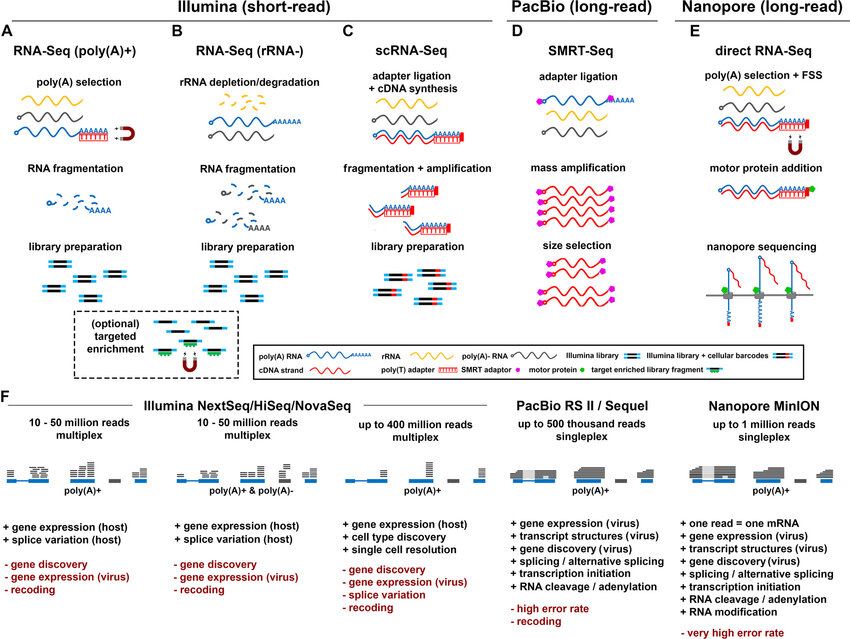
\includegraphics[width=\textwidth]{figures/biological_introduction/global_review_long_vs_short.png}
         \label{subfig:extensive-library-comparison}
         \caption[\textbf{Comprehensive comparison of RNA sequencing applications:}]{ \autocite[Fig. 1]{depledge_etal19}.}
     \end{subfigure}
   \caption[\textbf{Pros and cons of short-read (\Gls{illumina}) or long-read-based (PacBio and Nanopore) sequencing platforms}]{}
    \label{fig:rnaseq-libraries}
\end{figure}
The biological application of each sequencing platform will depend notably on the quality, the number and the averaged size of reads within (
\Cref{subfig:library-comparison-limitation} and \Cref{subfig:extensive-library-comparison}), for a detailled comparison on respective advantages and 
limitations offered by each library preparation strategy, see \autocite{head_etal14} and \autocite{stark_etal19}.
}}



\newglossaryentry{FASTA}
{name=FASTA, 
description={FASTA files gather a collection of sequences (a string of characters, 
such as A, U, G, C for RNA, that can span multiple lines and is not case-sensitive), 
each uniquely identified by a \emph{header line} 
(starting with symbol $>$, this line provides the name, source or any relevant context related to the sequence). 
FASTA files are easily readable by both humans and computational tools.}}

\newglossaryentry{cell marker}
{name=cell markers, 
description={Cells markers, expressed either on the cell surface or intracellular, (proteins, lipids, glycosylation, etc.) can be used to set apart unique cell types}}

\newglossaryentry{hematopoiesis}
{name=hematopoiesis, 
description={The general process describing the generation and the renewal of the blood cells}}

\newglossaryentry{backbone}
{name=backbone, 
description={In a protein, the \textit{backbone} refers to the main chain of amino acids, linked by peptide bonds. The backbone scaffold provides the structure, shape and stability of the protein. On the other hand, \textit{side chains} refers to the chemical functional groups attached to the backbone. The side chains are responsible for the ternary structure of proteins, providing it its unique chemical and functional identity.
}}

\newglossaryentry{epithelial}
{name=epithelium, 
description={The epithelium is one of the four types of tissues making up the organs of the body, along with the connective (support function), muscular and nervous components. 
Similarly to the frontiers of a country, they have a protective role against potential intruders (mucous tissues, skin) and an exchange role (transfer of nutrients to the blood in the digestive tract and transfer of oxygen while flushing away carbon dioxide in the respiratory tract). Finally, as main component of glands, they play a key role in maintaining the homeostasis, releasing hormones in the blood system.  
}}

\newglossaryentry{anti-ssa}
{name={Anti-SSA and anti-SSB}, 
description={Anti-SSA autoantibodies (anti-Sjögren's syndrome A-related autoantibodies) are antinuclear autoantibodies 
associated with many autoimmune diseases, such as systemic lupus erythematosus (SLE), 
Sjögren's syndrome (SS) \autocite{franceschini_cavazzana05} \autocite{goeb_etal07}, or rheumatoid arthritis (RA). Anti-Ro autoantibodies are often associated 
with autoantibody anti-La/SSB, displaying similar molecular structure \autocite{gleicher_elkayam13}.
}}

\newglossaryentry{interferon}
{name=inferferon signature, 
description={There are two main classes of interferons: type I IFNs and type II IFNs \autocite{lee_ashkar18} \autocite{platanias05}. While there are many distinct type I IFNs (including IFN-$\alpha$ and IFN-$\beta$) binding to the same cell surface receptor, there is only one type II IFN, IFN-$\gamma$, which binds to a distinct cell surface receptor. Type I and type II IFNs activate common and distinct STAT (signal transducer and activator of transcription) pathways, hereby playing an important role in regulating the expression of transcriptome and the intensity of the immune response. 
Traditionally, type I IFNs are linked to the humoral immune response \autocite{lebon_etal01}, namely the activation of B cells and the release of antibodies directly targeting foreign invaders, such as viruses or bacteria \autocite{zajac_harrington14}, whereas type II IFN is generally linked to the cell-mediated response \autocite{murray_etal02}. on the other hand, IFN type II activates the production of TCD4 and TCD8 cells, which in turn target self cells displaying aberrant phenotypic activity, resulting from viral infection or tumoral evolution.
 }}
 
 \newglossaryentry{serendipity}
{name=serendipity, 
description={Serendipity refers to fortunate discoveries performed by chance or accident.}
 }
 
  \newglossaryentry{linkage-disequilibrium}
{name=linkage disequilibrium, 
description={ Linkage disequilibrium refers to the genetic observation that alleles at different loci 
on a chromosome tend to be inherited together more often than expected by chance, implying that the genetic recombination 
during inheritance was not performed independently. This phenomena is usually triggered by the physical proximity of the linked variants
on the chromosome.
Notably, strong linkage disequilibrium may negatively impact bioinformatic analysis in the aforementionned cases:
\begin{itemize}
\item when conducting genome-wide association studies (GWAS), identifying Causal Variants responsible for 
a particular trait is much more challenging, since identify the one variant driver truly responsible for the observed effect
 is much harder in a set of highly related genetic variants due to strong LD, leading to numerous spurious associations.
 \item Similarly, it negatively impacts the sensibility of Genetic Risk Prediction, 
 since they assume that genetic variants are independently contributing to the risk of a disease. 
 Strong LD can violate this assumption, leading to overestimation or underestimation of the true risk.
 \item As detailled in \Cref{sec:drug-repurposing}, strong LD complicates the identification of drug targets based on GWAS,
 since the association between a gene and a disease may solely results from a nearby gene in the same LD region. Hence, it is crucial to
 validate biologically and clinically the putative targets, and prioritise them according to the level of credibility association.
\end{itemize}
To address these challenges, additional functional studies, fine-mapping of the local genetic environment, causal analyses and
 integration of other genomic data are often needed to pinpoint the causal variants.}
 } 
 
 \newglossaryentry{cross-sectional}
{name=cross sectional, 
description={Cross-sectional studies gather data from multiple subjects at a specific time point,
 whereas longitudinal studies collect data from the same subjects over multiple time points, 
 often concentrating on a smaller group of individuals with similar biological patterns.  
 The differences between the two experimental trial designs is schematically represented in \Cref{fig:cross-study} 
 \begin{figure}[b]
\centering
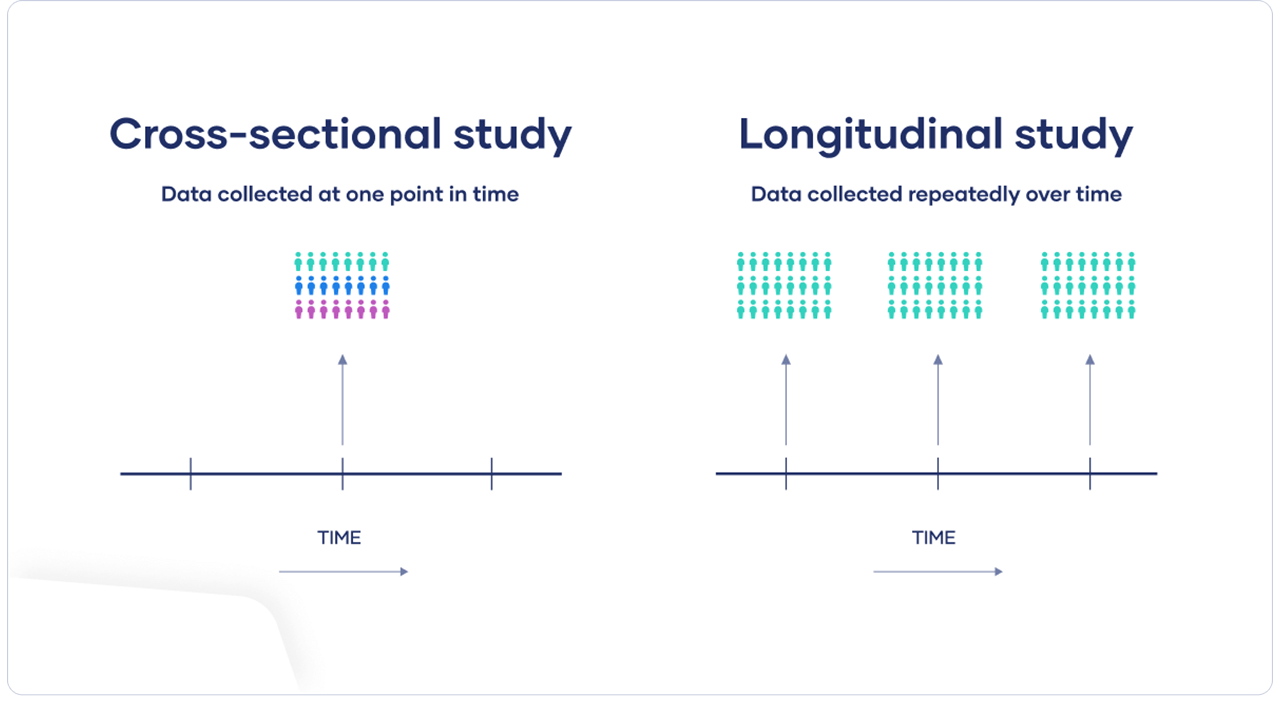
\includegraphics[width=0.8\textwidth]{figures/sjogren/sectional-vs-long.png}
\caption{Visual representation of cross-sectional and longitudinal studies differences, from \autocite{louis23}.}
\label{fig:cross-study}
\end{figure}
 }}
 






